\subsection{Counter}

\begin{figure}[htbp]
   \centering
   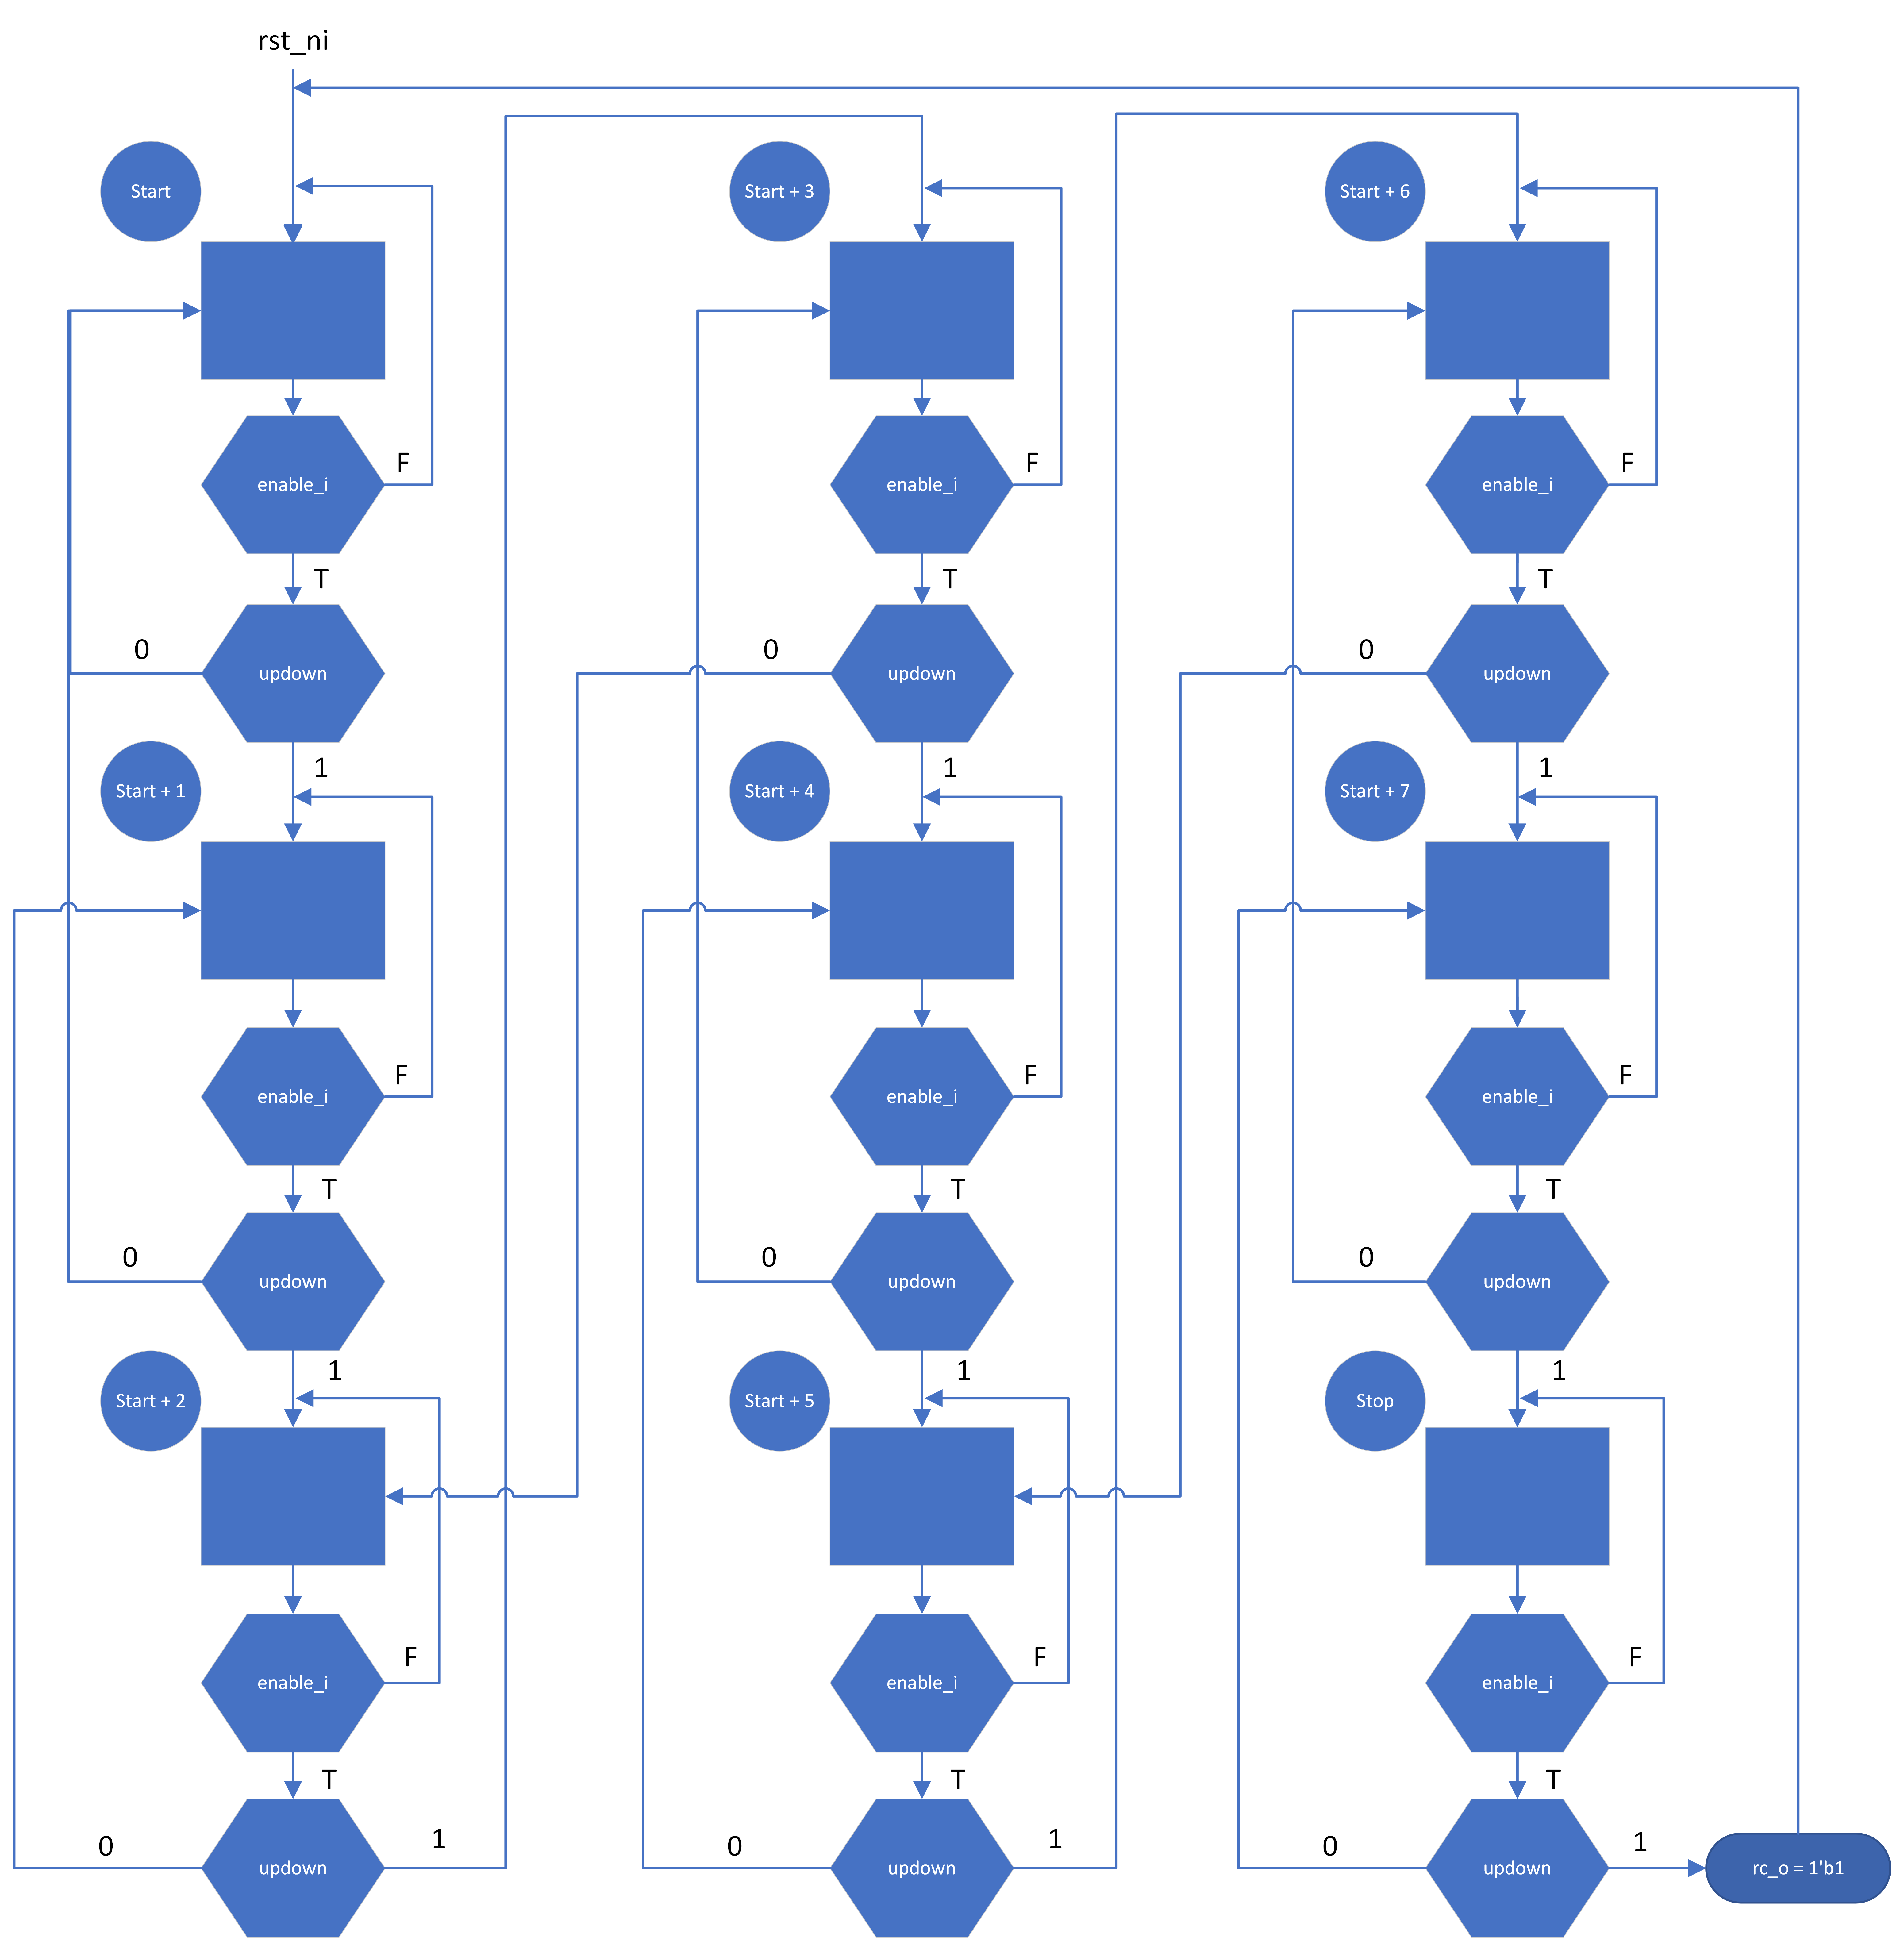
\includegraphics[width=\textwidth]{counter_asm.png}
   \caption{ASM chart of the counter module.}
   \label{fig:counter_asm}
\end{figure}

\begin{minted}[
   fontsize=\footnotesize,
   linenos,
   breaklines,
]{verilog}
module counter (
   input clk_i,
   input rst_ni,
   input ena_i,
   input updown_i,
   output reg [3:0] cnt_o
);

always @(posedge clk_i, negedge rst_ni)
   if (!rst_ni)
      cnt_o <= 4'b0;
   else if (!ena_i)
      cnt_o <= cnt_o;
   else
      if (updown_i)
         if (cnt_o == 4'd9)
            cnt_o <= 4'b0;
         else
            cnt_o <= cnt_o + 1'b1;
      else
         if (cnt_o == 4'd0)
            cnt_o <= 4'd9;
         else
            cnt_o <= cnt_o - 1'b1;

endmodule
\end{minted}

\begin{minted}[
   fontsize=\footnotesize,
   linenos,
   breaklines,
]{verilog}
module counter_tb;

// Inputs
reg clk;
reg rst_n;
reg ena_i;
reg updown_i;

// Outputs
wire [3:0] cnt_o;

counter DUT (
   .clk_i(clk),
   .rst_ni(rst_n),
   .ena_i(ena_i),
   .updown_i(updown_i),
   .cnt_o(cnt_o)
);

// Create a 50Mhz clock
always #10 clk = !clk;  // every ten nanoseconds invert

initial begin
   clk = 1'b0;
   rst_n = 1'b0;
   ena_i = 1'b0;  // disabled
   updown_i = 1'b1;  // count up
end

initial begin
   #20 rst_n = 1'b1;  // release reset

   // Test 0 -> 9
   @(posedge clk);
   ena_i = 1'b1;
   @(posedge clk);
   ena_i = 1'b0;
   updown_i = 1'b0;
   @(posedge clk);
   ena_i = 1'b1;
   @(posedge clk);
   ena_i = 1'b0;
   @(posedge clk);
   ena_i = 1'b1;
   @(posedge clk);
   ena_i = 1'b0;

   // Test 9 -> 0
   updown_i = 1'b1;
   @(posedge clk);
   ena_i = 1'b1;
   @(posedge clk);
   ena_i = 1'b0;
   @(posedge clk);
   ena_i = 1'b1;
   @(posedge clk);
   ena_i = 1'b0;

   // Test reset
   @(posedge clk);
   ena_i = 1'b1;
   @(posedge clk);
   ena_i = 1'b0;
   @(posedge clk);
   ena_i = 1'b1;
   @(posedge clk);
   ena_i = 1'b0;
   @(posedge clk);
   rst_n = 1'b0;
   @(posedge clk);
   rst_n = 1'b1;

// Finish the Simulation
   #100;
   $finish;
end

endmodule
\end{minted}

\begin{figure}[htbp]
   \centerline{
   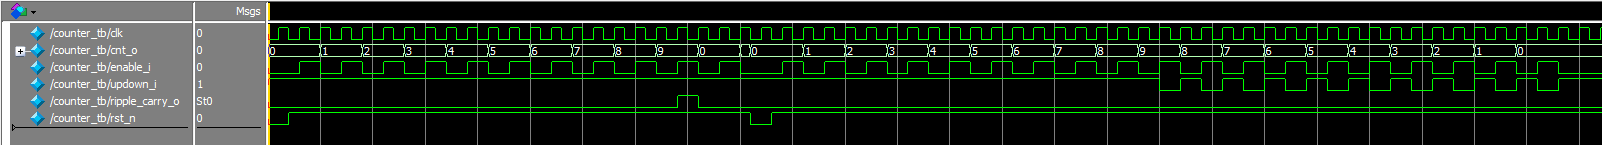
\includegraphics[width=\paperwidth]{counter_sim.png}}
   \caption{Testbench simulation of the counter module.}
   \label{fig:counter_sim}
\end{figure}

Fig.~\ref{fig:counter_sim} shows the simulation test results of the counter module. The counter counts up when updown is high potential and counts down when it is low potential. The enable signal triggers the counter to count once.

The first test case was to count from nine to zero. Nine set to the biggest digit this counter can count to. The second test case was to count beyond nine, which returned the count to zero. Next, Reset singal reset the count to zero.
